\chapter{Relation with Wizard of Oz}\label{chap:woz}

\graphicspath{{images/woz/}}

\begin{framed}
	\textbf{Key points:}
	
	\begin{itemize}
		\item An experiment was designed to explore the influence of \gls{sparc} on the human workload and task performance compared to an approach based on \gls{woz}.
		\item Application target replaced by a robot to ensure repeatability of target behaviour.
		\item Design of a robot model exhibiting probabilistic behaviour with a non-trivial optimal interaction policy.
		\item Results show that \gls{sparc} achieves a similar performance than \gls{woz} while requiring a lower workload from the teacher.
	\end{itemize}
\end{framed}

Parts of the work presented in this chapter have been published in \cite{senft2015sparc} \footnote{Note about technical contribution in this chapter: the author used software from the \gls{dream} project for the touchscreen and the robot functionalities. The author contributed to the material used within the robot control and the Graphical User Interface. Algorithm used from the OPENCV neural network library.} . The final publication is available from Springer via \url{http://dx.doi.org/10.1007/978-3-319-25554-5_60}.

\newpage

\section{Motivation}

\gls{sparc} as been designed to enable end-users non-experts in computer science to teach a robot an action policy while interacting in a sensitive environment. The argument behind this way of interacting is that \gls{sparc} allows a field expert to transfer their knowledge to an autonomous agent without having to enforce each actions manually. Additionally, as the agent is interacting in the target environment, displaying a appropriate action policy, the time spend to teach it is not lost as the desired interaction takes place also during the learning phase. For example, using the context of \gls{rat}, a therapist would teach the robot during a therapy session. As the therapist is in total control of the robot's action, the behaviour expressed by the robot fits the  behaviour desired for the therapy ensuring that even the sessions used to teach the robot have a therapeutic value for the patient involved in the therapy.

\gls{sparc}, as a principle, allows to start a robotic application in a \gls{woz} fashion and then move away from it as the robot gains autonomy. The aim of \gls{sparc} is twofold: maintaining a high level of performance in the target application while reducing the workload of the teacher over time. As the robot learns, the action policy is refine until reaching a point where the robot is autonomous or only necessitates minimal supervision to interact successfully. As explained in Chapter \ref{chap:sparc}, \gls{sparc} involves two interactions the control interaction and the application one. And when the goal is learning how to interact with humans, the robot is interacting simultaneously with at least two humans. These two dependent interactions complexify the evaluation of the approach, especially as both humans are impacting each other. The first step to evaluate \gls{sparc} was to focus on the relation between the robot and its teacher. To evaluate this aspect of the interaction, we decided use the context of a \gls{rat} for children, but replacing the child involved in the therapy by a robot running a model of a child. The setup ends up with two robots interacting together: the child-robot completing a task and the wizarded-robot, controlled by a participant, supporting the child-robot in its task completion. The child-robot behaviour is impacted by the other robot's action, and a child-robot reaching a high performance would indicate that the supporting policy of the wizarded-robor is efficient, demonstrating the capability of the human in the supervision. This allows us to observe the impact of \gls{sparc} on the teacher in a repeatable environment. 

\section{Scope of the study}

This study aims to evaluate if \gls{sparc} can allow a human to teach a robot an efficient action policy in a human-robot interaction modelled by two robots interacting together. The control condition is a variation of \gls{woz} and by providing a learning component to the robot, \gls{sparc} aims to allow the teacher to maintain a high performance during the interaction while reducing the workload on the teacher over time.

To evaluate the validity of \gls{sparc} and the influence of such an approach, four hypotheses were devised:
\begin{enumerate}
	\item [H1] The child-robot's performance is a good proxy for the teacher's performance.
	\item [H2] When interacting with a new system, humans progressively build a personal strategy that they will use in subsequent interactions.
	\item [H3] Reducing the number of interventions required from a teacher reduces their perceived workload.
	\item [H4] Using \gls{sparc} allows the teacher to achieve similar performance than \gls{woz} but with a lower workload.
\end{enumerate}

H1 represents a sanity check for the model, ensuring that the child-robot performance represents the efficiency of the action policy applied by the teacher. H2 tests that human teachers are not static entities, they adapt their learning target and their teaching strategy. H3 tests one of the motivations behind \gls{sparc}: does reducing the number of physical actions from a human to control a robot while requiring the teacher to monitor the robot suggestions lead to a lower workload. And finally, H4 is the main hypothesis, does \gls{sparc} enables a robot to learn a useful action policy: reducing the teacher's workload while maintaining a high performance.

\section{Methodology}

This study is based on a real scenario for \gls{rat} for children with \gls{asd} based on the Applied Behaviour Analysis therapy framework \citep{cooper2007applied}. The aim of the therapy is to help a child to develop/practice their social skills. The child has to complete an emotion recognition task by playing a categorisation game with a robot on a mediating touchscreen device \citep{baxter2012touchscreen}. And the robot can provide feedback and prompts to encourage the child and help them to classify emotions. The task is the following: images of faces or drawings are shown to the child on the touchscreen, and the child has to categorise them by moving them to one side of the screen or the other depending on whether the picture shown denotes happiness or sadness. In the therapy, the robot is remote-controlled by an operator using the \acrlong{woz} paradigm.%, and does not interact with the child directly. 

This study explores if \gls{sparc} can be used to teach the robot a correct action policy to support the child in this therapy scenario. As timing in human-robot interactions is complex, for simplification reasons, the interaction has been discretised to have clear steps when the robot has to select an action. During these action steps, the selection of an action is decided by following the principles defining the \gls{sa}:
\begin{enumerate}
	\item The robot suggests an action to the teacher.
	\item The teacher can select an action for the robot to execute or let the proposed action be executed after a short delay.
	\item The robot executes the selected action.
	\item Both robot and teacher observe the outcome of the action until the next action selection step.
\end{enumerate}

Using \gls{sparc}, the robot learns over time to replicate the teacher's policy by matching the inputs (child's state) to the outputs (action selected by the teacher). 

%the policy used by the teacher based on observations of the child and the oversight from the teacher, with the teacher still maintaining overall control if necessary.

Two conditions are compared: \gls{sparc}, where the robot learns from the human corrections and the \gls{woz} condition. To maintain comparability between the two conditions, with \gls{woz} the robot proposes random actions instead of learnt actions increasing the probability of having the teacher correcting the suggestion to have a setup closer to a real \gls{woz}.

The focus of the study being on the teaching interaction (the relation between the teacher and the robot), the second interaction (the application one) has been kept constant by replacing the child by a robot. A minimal model of child behaviour is therefore used to stand in for a real child. A second robot is employed in the interaction to embody this child model: we term this robot the \textit{child-robot} while the robot being directly supervised by the human teacher is the \textit{wizarded-robot} (Figure \ref{fig:woz_setup}).

\begin{figure}[ht]
	\centering
	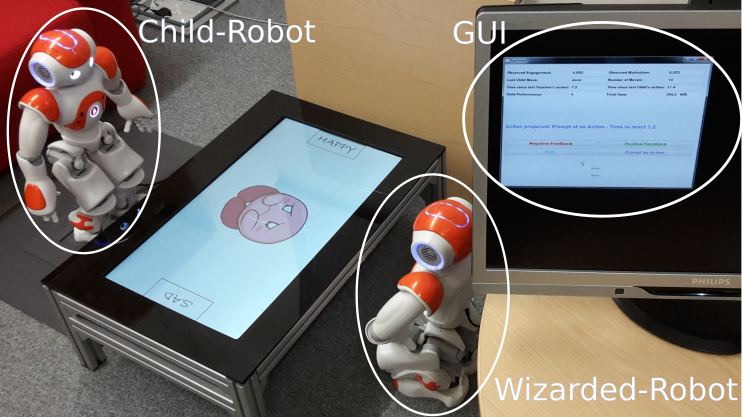
\includegraphics[width=.9\textwidth]{setup_annotated.png}
	\caption{Setup used for the user study from the perspective of the human teacher. The child-robot (left) stands across the touchscreen (centre-left) from the wizarded-robot (centre-right). The teacher can oversee the actions of the wizarded-robot through the \gls{gui} and intervene if necessary (right).}
	\label{fig:woz_setup}
\end{figure}
		
\subsection{Child model} \label{ssec:woz_child}

The purpose of the child model is not to realistically model a child (with or without autism), but to provide a means of expressing some characteristics of the behaviours we observed in interactions with children in a repeatable manner. The child-robot possesses an internal model encompassing an engagement level and a motivation level, together forming the state of the child. The engagement represents how often the child-robot will make categorisation moves and the motivation gives the probability of success of the categorisation moves. These states are bound to the range [-1, 1] and influenced by the behaviour of the wizarded-robot, and will asymptotically decay to zero with no actions from the wizarded-robot. These two states are not directly accessed by either the teacher or the wizarded-robot, but can be observed through behaviour expressed by the child-robot: low engagement will make the robot look away from the touchscreen, and the speed of the categorisation moves is related to the motivation (to which gaussian noise was added). There is thus incomplete/unreliable information available to both the wizarded-robot and the teacher.

The influence of the wizarded-robot behaviour on the levels of engagement and motivation are described below (Section \ref{ssec:woz_wizarded_robot}). In addition to this, if a state is already high and an action from the wizarded-robot should increase it further, then there is a chance that this level will sharply decrease, as an analogue of frustration. When this happens, the child-robot will indicate this frustration verbally (uttering one of eight predefined strings). This mechanism prevent the optimal strategy to be straightforward: always making actions aiming to increase motivation or engagement. The optimal strategy combines feedback actions and waiting ones to maintain the state values high but prevent them to overshoot. This non-trivial optimal action policy approximates better a real human-robot interaction scenario requiring a more complex strategy to be expressed by the robot.

\subsection{Wizarded-robot control}
\label{ssec:woz_wizarded_robot}
The wizarded-robot is controlled through a \gls{gui} (shown in Figure \ref{fig:woz_gui}) and has access to the variables defining the state of the interaction used by the learning algorithm:
\begin{itemize}
	\item Observed engagement
	\item Observed motivation
	\item Type of last move made by the child-robot (good/bad/done)
\end{itemize}

\begin{figure}[ht]
	\centering
	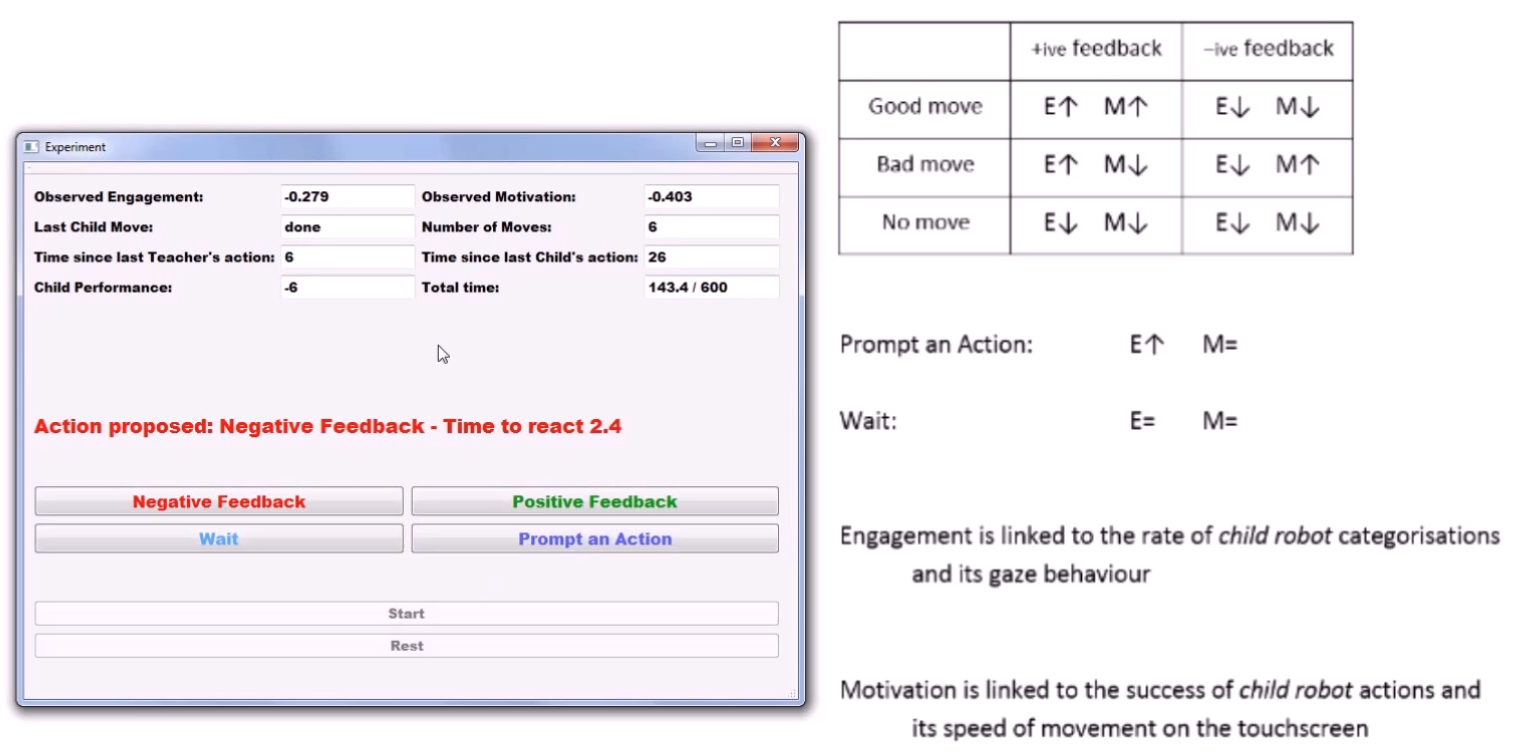
\includegraphics[width=.9\textwidth]{GUI-woz.png}
	\caption{Screen shot of the interface used by the participants, the \gls{gui} on the left allows to control the robot and a summary of the actions' impact is displayed on the right.}
	\label{fig:woz_gui}
\end{figure}

Additionally, other metrics are displayed to the teacher but not used by the algorithm:
\begin{itemize}
	\item Number of categorisations made by the child-robot
	\item Time since last teacher's action
	\item Time since last child's action
	\item Child's performance
	\item Total time elapsed
\end{itemize}


The wizarded-robot has a set of four actions, with one button each on the \gls{gui}: 
\begin{itemize}
	\item Prompt an Action: Encourage the child-robot to do an action.
	\item Positive Feedback: Congratulate the child-robot on making a good classification.
	\item Negative Feedback: Supportive feedback for an incorrect classification.
	\item Wait: Do nothing for this action opportunity, wait for the next one.
\end{itemize}


The impact of actions on the child-robot depends on the internal state and the type of the last child-robot move: good, bad, or done (meaning that feedback has already been given for the last move and supplementary feedback is not necessary). A \textit{prompt} increases the engagement, a \textit{wait} has no effect on the child-robot's state, and the impact of positive and negative feedback depends on the previous child-robot move. Congruous feedback (positive feedback for correct moves; negative feedback for incorrect moves) results in an increase in motivation, but incongruous feedback can decrease both the motivation and the engagement of the child-robot. The teacher therefore has to use congruous feedback and prompts.

However, as mentioned in Section \ref{ssec:woz_child}, if the engagement or the motivation exceeds a threshold, their value can decrease abruptly to simulate the child-robot being frustrated. This implies that the optimal action policy provides congruous feedback and prompts, but also requires wait actions to prevent the child-robot becoming frustrated and keep its state-values close to the threshold without exceeding it. A `good' strategy keeping the engagement and motivation high leads to an increase in performance of the child-robot in the categorisation task.

As introduces previously, to simplify the algorithm part, the interaction has been discretised, the teacher can not select actions for the wizarded-robot at any time, actions can only be executed at specific times triggered by the wizarded-robot: two seconds after each child-robot categorisation or if nothing happened for five seconds since the last wizarded-robot action. When these selection windows are hit, the wizarded-robot proposes an action to the teacher by displaying the action's name and a countdown before execution. The teacher can only select an action in reaction to a proposition from the wizarded-robot; alternatively, if the teacher does nothing in the three seconds following the suggestion, the action proposed by the wizarded-robot is executed. This mechanism allows the teacher to passively accept a suggestion or actively make an \emph{intervention} by selecting a different action and forcing the wizarded-robot to execute it.

\subsection{Learning algorithm}

In the \gls{sparc} condition, the robot learns to reproduce the action policy displayed by the teacher. For this study, the robot learns using a Multi-Layer Perceptron (MLP): with five input nodes: one for the observed motivation, one for the observed engagement and three binary (+1/-1) inputs for the type of the previous move: good, bad, or done. The hidden layer had six nodes and the output layer four: one for each action. The suggested action is selected applying a Winner-Take-All strategy on the value of the output node and then displayed on the \gls{gui} before execution. The network is trained with back propagation: after each new decision from the teacher a new training point is added with the selected action node having +1 while the others -1. The network is fully retrained with all the previous state-action pairs and the new one between each selection step. 
%The network was using sigmoid activation function and a learning rate of 0.6 (probably).

This learning algorithm, MLP, is not optimal for a real time interaction as the online learning should happens quickly between learning iteration. However as the length of interaction (and so the number of datapoints) is limited, the action selection rate is low and the desired learning behaviour is purely supervised learning, this type of algorithm has been deemed suitable for this study.
%On the other side, the random controller proposed random actions to the teacher.

\subsection{Participants}

In \gls{rat} scenarios using \gls{woz} to control the robot, the wizard is typically a technically competent person with previous experience controlling robots or at least significant training controlling this robot for the therapy. As such, to maintain consistency with the target user group, the participants of this study (assuming the role of the teacher) have been taken from a robotics research group. Ten participants were used (7M/3F, age \textit{M}=29.3, 21 to 44, \textit{SD}=4.8 years).

\subsection{Interaction Protocol}

The study compared two conditions: a learning robot adapting its propositions to its user (the \gls{sparc} condition) and a non-learning robot constantly proposing random actions (the \gls{woz} condition). The child-robot controller was kept constant in both conditions, while the state is reset between interactions. The design was a within subjects comparison with balancing of order: each participant interacted with both conditions, with the order balanced between participants to control for any ordering effects. In the order LN the participants first interact with the learning wizarded-robot in the \gls{sparc} condition, and then with the non-learning one in the \gls{woz} condition; in the order NL, this interaction order is inverted. Participants were randomly assigned to one of the two orders.

The interactions took place on a university campus in a dedicated experiment room. Both robots were Aldebaran Nao, one of which had a label indicating that it was the child-robot. The robots faced each other with a touchscreen between them, and participants assuming the role of the teacher sat at a desk to the side of the wizarded-robot, with a screen and a mouse to interact with the wizarded-robot (fig. \ref{fig:woz_setup}). Participants were able to see the screen and the child-robot.

A document explaining the interaction scenario was provided to participants with a demographic questionnaire\footnote{Questionnaires and information sheet can be found at \url{https://emmanuel-senft.github.io/experiment-woz.html}}. After the information had been read, a 30s video presenting the \gls{gui} in use was shown to familiarise the participants with it, without biasing them towards any particular control strategy. Then participants clicked a button to start the first interaction which lasted for 10 minutes. The experimenter was sat in the room outside of the participants' field of view. After the end of the first interaction, a post-interaction questionnaire was administered. Similarly, in the second part of the experiment, the participants interact with the other condition and complete a second post-interaction questionnaire. Finally, a post-experiment questionnaire asked participants to explicitly compare the two conditions.

\subsection{Metrics}

Two types of metrics have been recorded for this study: interaction data representing objective behaviours and performance of the participants and subjective data through questionnaires.

\subsubsection{Interaction data}

The state of the child-robot and the interaction values were logged at each step of the interaction (at 5Hz). All of the human actions were recorded: acceptance of the wizarded-robot's suggestion, selection of another action (intervention), and the states of the child-robot (motivation, engagement and performance) at this step. 

The first metric is the performance achieved by participants in each interaction. As the policy applied by the participants cannot be evaluated directly, the performance of the child-robot in the task (number of correct categorisations minus number of incorrect categorisations ) is used as a proxy for the participant performance. And H1 evaluates if this approximation is valid by analysing the relation between the performance of the child-robot and the value of its inner states. If a correlation is found, it would demonstrate that a good supervision policy (managing to keep the engagement and the motivation of the child-robot high) leads to a high performance. And, as such, this child-robot performance represents how efficient the action policy executed by the wizarded-robot was when controlled by a participant.

The second important metric is the intervention ratio: the number of times a user chooses a different action than the one proposed by the wizarded-robot, divided by the total number of executed actions. This metric represents how often in average a user had to correct the robot and could be related to the workload the user had to face to control the robot.

\subsubsection{Questionnaire data}
 
Participants answered to four questionnaires: a demographic one, before the interaction, two post-interaction ones where they were asked to evaluate the last interaction with the robots and a post-experiment where they had to compare the two conditions. All the rating questionnaires used seven items Likert scale and in the questionnaires the wizarded-robot is named the `teacher-robot'.

Post-Interaction questions:
\begin{itemize}
	\item The child-robot learned during the interaction.
	\item The performance of the child-robot improved in response to the teacher-robot actions.
	\item The teacher-robot is capable of making appropriate action decisions in future interactions without supervision.
	\item The teacher-robot always suggested an incorrect or inappropriate actions.
	\item By the end of the interaction, my workload was very light.
	\item What did you pay most attention during the interaction? (child-robot, touchscreen, \gls{gui}, other).
\end{itemize}

Post-experiment questions:
\begin{itemize}
	\item There was a clear difference in behaviour between the two teacher-robots.
	\item There was a clear difference in behaviour between the two child-robots.
	\item Which teacher-robot was better able to perform the task? (first, second).
	\item Which teacher-robot did you prefer supervising? (first, second).
\end{itemize}

\section{Results}

\subsection{Interaction data}

Figure \ref{fig:woz_comp} presents the aggregated results (collapsed between orders) for the performance and the final intervention ratio for both conditions. While the number of participants are not sufficient to perform statistical comparison, overall interaction results seem to show that both conditions lead to similar performance (\gls{sparc}: 32.6 (95\% CI [27.89,37.31]) - \gls{woz}: 31.4 (95\% CI [25.9,36.9])) while the \gls{sparc} condition required less intervention (intervention ratio: \gls{sparc}: 0.38 (95\% CI [0.29,0.47]) - \gls{woz}: 0.59 (95\% CI [0.52,0.67])). 

\begin{figure*}[ht]
	\centering
	\begin{subfigure}[ht]{0.5\textwidth}
		\centering
		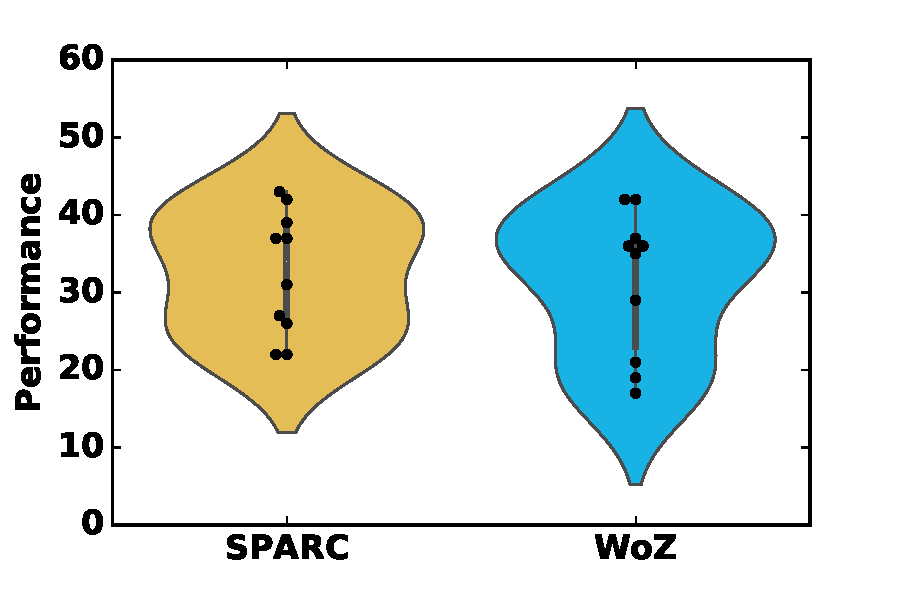
\includegraphics[width=1.0\textwidth]{perf.pdf}
%		\caption{Comparison of end performance for both conditions.}
	\end{subfigure}%
	~ 
	\begin{subfigure}[ht]{0.5\textwidth}
		\centering
		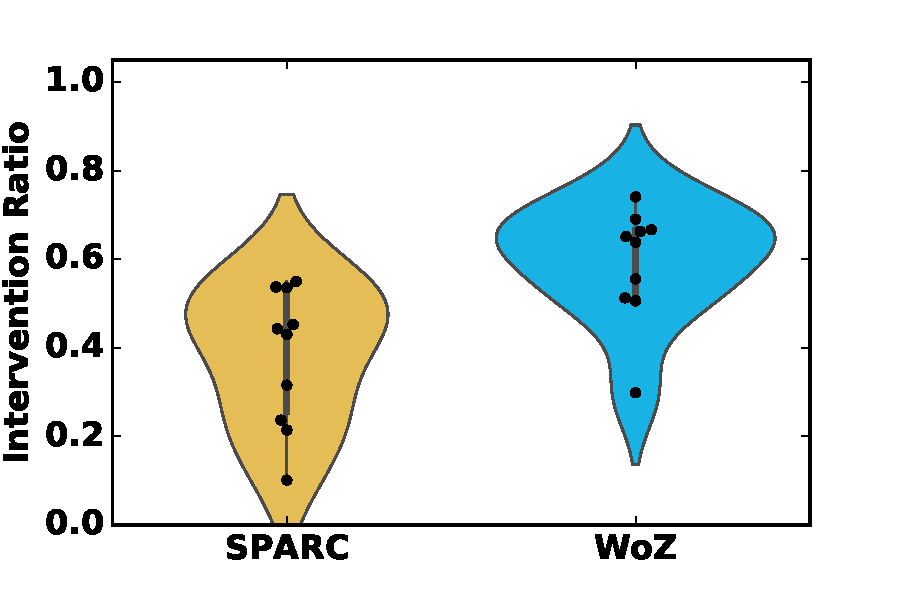
\includegraphics[width=1.0\textwidth]{ratio.pdf}
%		\caption{Comparison of intervention ratio for both conditions.}
	\end{subfigure}
	\caption{Aggregated comparison of performance and final intervention ratio for both conditions}
	\label{fig:woz_comp}
\end{figure*}

Figure \ref{fig:woz_ratio_time} presents the evolution of intervention ratio for each condition and orders. During the first interaction, participants discover the interface and how to interact with it, which results in a high variation intervention ratio in the first 20 steps (each time the wizarded-robot proposes an action). However in the second phase of the interaction,  when participants develop their teaching policy, there is a tendency of \gls{sparc} requiring a lower number of intervention than \gls{woz}. This effect is higher in the second interaction, where as soon as 5 steps, the two conditions differentiate without overlap of the 95\% CI of the mean, which would indicate that the two conditions differ in term of required interventions.

\begin{figure}[ht]
	\centering
	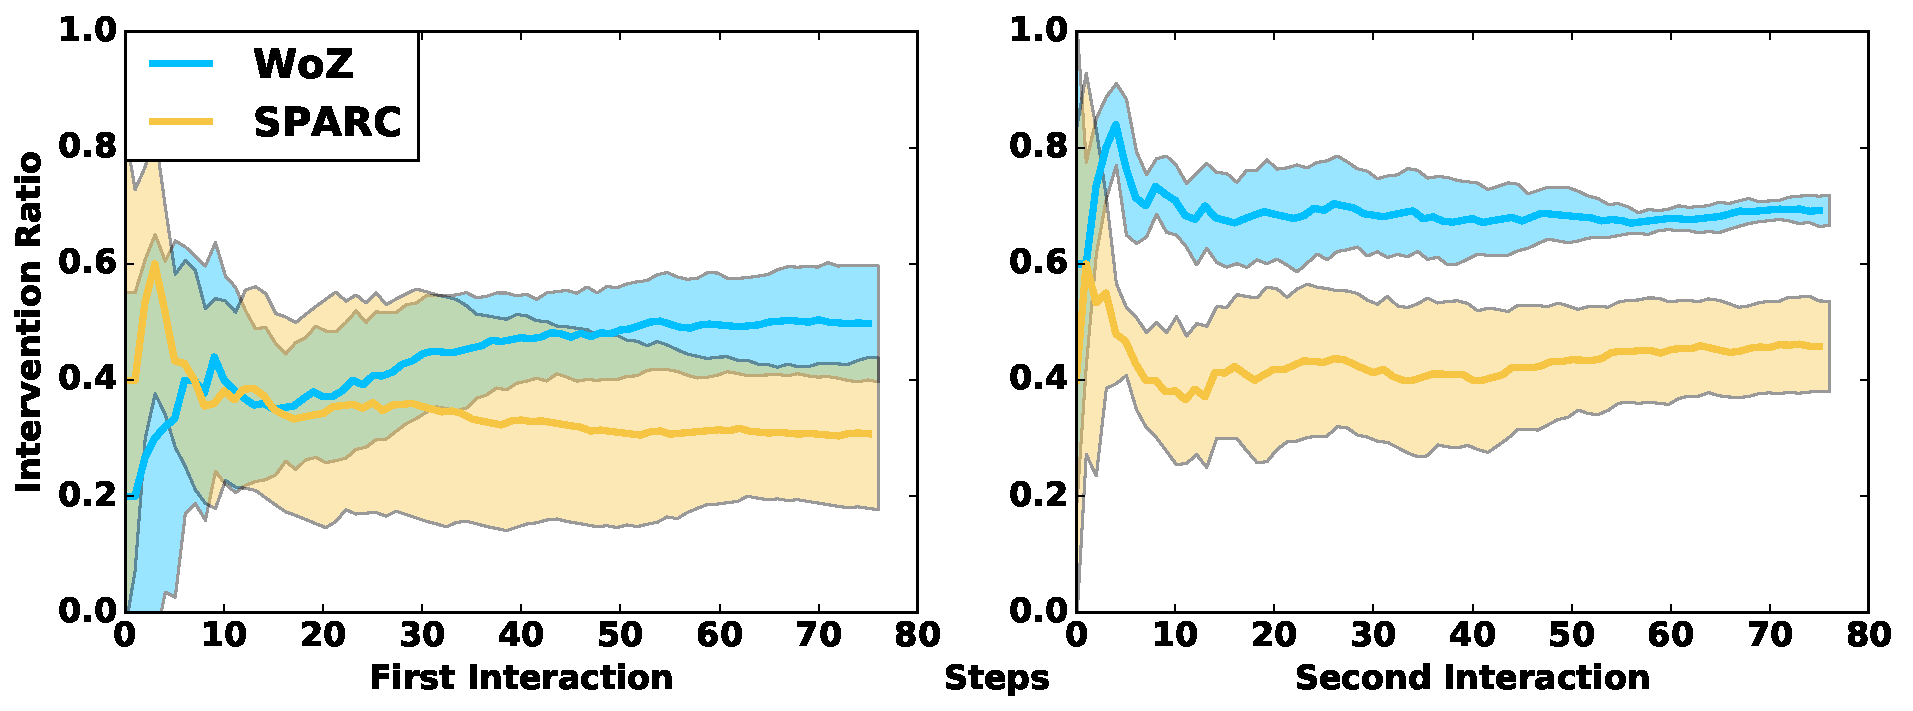
\includegraphics[width=1.\textwidth]{ratio_time.pdf}
	\caption{Evolution of intervention ratio over time for both conditions and both orders. Shaded area represents the 95\% CI.}
	\label{fig:woz_ratio_time}
\end{figure}

Both for the performance and the intervention ratio, a strong ordering effect have been observed. Figure \ref{fig:woz_separated} and Table \ref{tab:woz_comp_means} present the performance and final intervention ratio separated by condition and order. In both orders, the second interaction has higher performance as the participants were used to the system and understood how to develop an efficient interaction policy, while the performance between condition for the same interaction number is similar. However, regardless of the order, when only the interaction number is considered, the intervention ratio is lower when using \gls{sparc} compared to \gls{woz}. This indicates that when the wizarded-robot learned using \gls{sparc}, a similar performance is attained as with \gls{woz}, but the number of interventions required to achieve this performance is lower.

%COuld use the CIDM if desired or not

\begin{figure}[ht]
	\centering
	\begin{subfigure}[t]{0.5\textwidth}
		\centering
		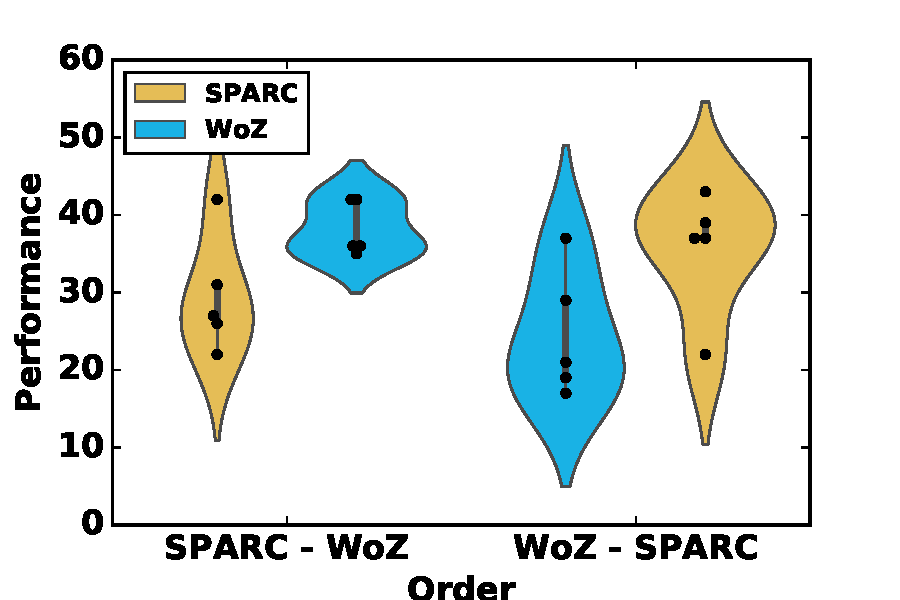
\includegraphics[width=1.\textwidth]{perf_divided.pdf}
	\end{subfigure}%
	\begin{subfigure}[t]{0.5\textwidth}
		\centering
		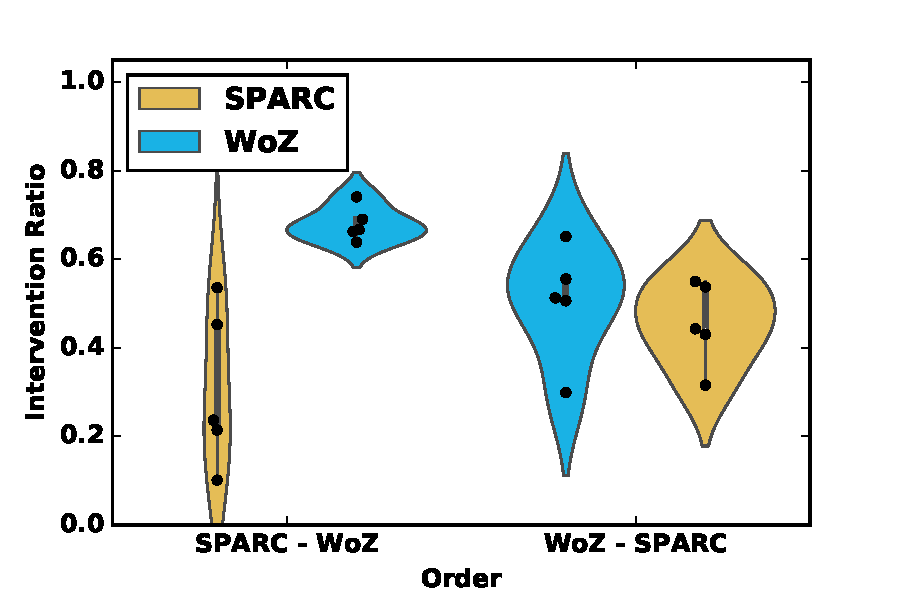
\includegraphics[width=1.\textwidth]{ratio_divided.pdf}
	\end{subfigure}
	\caption{Performance achieved and final intervention ratio separated by order and condition. For each order, the left part presents the metric in the first interaction (with one condition) and the right part the performance in the second interaction (with the other condition).}
	\label{fig:woz_separated}
\end{figure}


\begin{table}[t]
	\caption{Average performance and intervention ratio separated by condition and order.}
	\centering
\begin{tabulary}{1.0\textwidth}{L"C|C"C|C}
	& \multicolumn{2}{c"}{Order LN} & \multicolumn{2}{c}{Order NL} \\
	& \gls{sparc} (int 1) & WoZ (int 2) & WoZ (int 1) & \gls{sparc} (int 2) \\
	\hline			
Performance M \linebreak 95\% CI & 29.6 [23.61,35.59] & 38.2 [35.46,40.94] & 24.6 [18.1,31.1] & 35.6 [29.34,41.86]\\
Intervention Ratio M 95\% CI & 0.31 [0.17,0.45] & 0.68 [0.65,0.71] & 0.5 [0.4,0.61] & 0.46 [0.38,0.53]\\
\end{tabulary}
\label{tab:woz_comp_means}
\end{table}



%In both conditions, the average performance in the second interaction (\textit{M$_{LN-2}$} =38, 95\% CI [36.2, 39.8], \textit{M$_{NL-2}$}=34.8, 95\% CI [30.8, 38.8]) was higher than in the first one (\textit{M$_{LN-1}$}=29.4, 95\% CI [25.3, 33.5], \textit{M$_{NL-1}$}=24.3, 95\% CI [19.4, 29.4]; Fig. \ref{fig:graphs} \textit{left}). The 95\% \textit{Confidence Interval of the Difference of the Mean} (CIDM) for the L-NL condition is [4.1, 13.1] and for the NL-L condition is [4.0, 16.8].
%However, the performance is similar when only the interaction order (first or second) is considered. 
%The participants performed slightly better in the LN condition, but the CIDM includes zero in both cases (95\% CIDM$_{1}$ [-1.5, 11.5], 95\% CIDM$_{2}$ [-1.2, 7.6]). 
%In the condition L-NL, the intervention ratio increased between the learning and non learning condition (\textit{M$_{LN-1}$}=0.31, 95\% CI [0.20, 0.42] to \textit{M$_{LN-2}$}=0.68, 95\% CI [0.66, 0.70], CIDM$_{LN}$=[0.26, 0.48]). 
%But in the NL condition, the intervention ratio is almost identical between the two interactions but slightly lower for the learning case (\textit{M$_{NL-1}$}=0.50, 95\% CI [0.44, 0.57] to \textit{M$_{NL-2}$}=0.46, 95\% CI [0.40, 0.51], CIDM$_{NL}$ [-0.03, 0.13]).

Additionally, a strong positive correlation (Pearson's \textit{r}=0.79) was found between the average child-robot motivation and engagement and its performance which shows that the performance achieved by the child-robot represents the capacity of the teacher to keep both engagement and motivation high.

\subsection{Questionnaire data}

The post-interaction questionnaires evaluated the participant's perception of the child-robot's learning and performance, the quality of suggestions made by the wizarded-robot, and the experienced workload. All responses used seven point Likert scales.

Table \ref{tab:woz_quest_means} presents separated results for the questions asked in the post-interaction questionnaires, with more details for the questions exhibiting differences in Figure \ref{fig:woz_quest}.

\begin{figure}[ht]
	\centering
	\begin{subfigure}[t]{0.3295\textwidth}
		\centering
		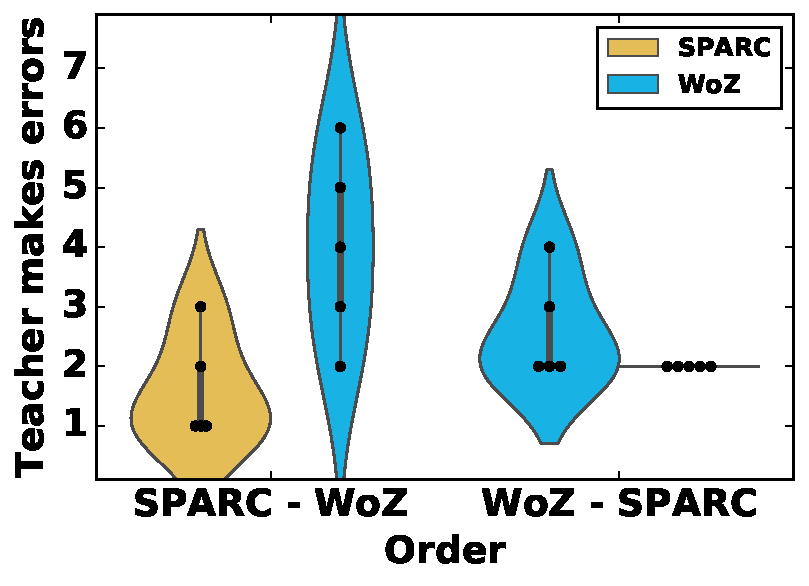
\includegraphics[width=1.\textwidth]{errors.pdf}
	\end{subfigure}%
	~ 
	\begin{subfigure}[t]{0.341\textwidth}
		\centering
		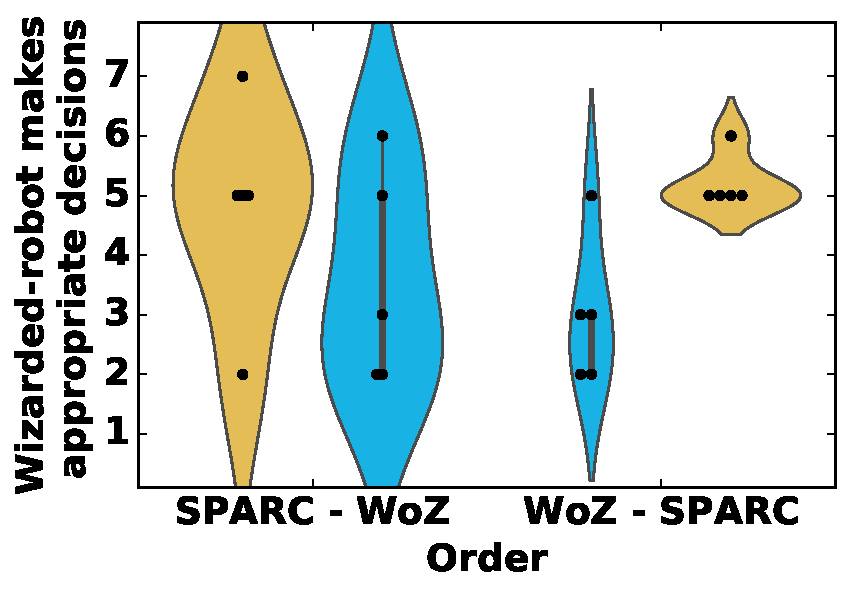
\includegraphics[width=1.\textwidth]{appropriate.pdf}
	\end{subfigure}%
	~ 
	\begin{subfigure}[t]{0.3295\textwidth}
		\centering
		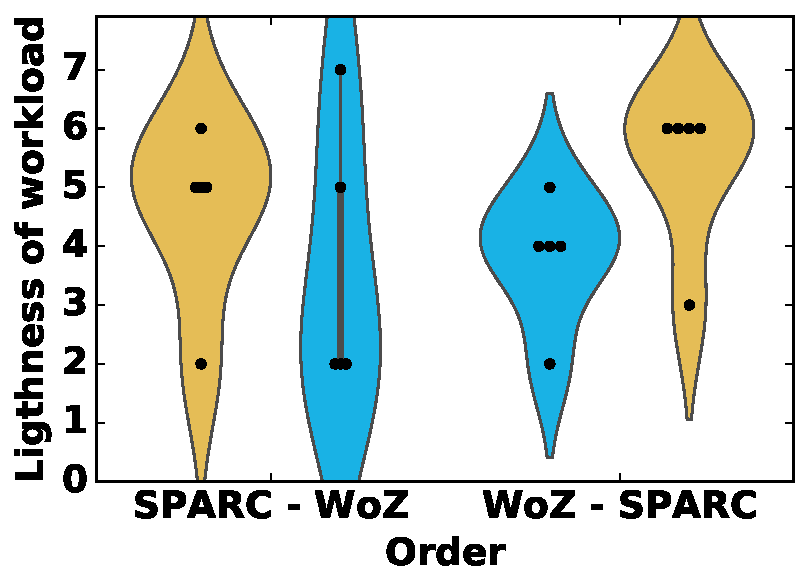
\includegraphics[width=1.\textwidth]{workload.pdf}
	\end{subfigure}
	\caption{Questionnaires results on robot making errors, making appropriate decisions and on lightness of workload.}
	\label{fig:woz_quest}
\end{figure}

Across the four possible interactions, the rating of the child-robot's learning was similar (\textit{M}=5.25, 95\% CI [4.8, 5.7]). As the child-robot was using the same interaction model in all four conditions, this result is expected. There is a slight tendency to rate the child's performance as being higher in the \gls{woz} condition but the error margin is too high to conclude anything. %This could indicate that the teachers were more aware of the child's behaviour as the workload was lighter to control the wizarded-robot.

\begin{table}[t]
	\caption{Average reporting on questionnaires separated by condition and order.}
	\centering
	\begin{tabulary}{1.0\textwidth}{L"C|C"C|C}
		& \multicolumn{2}{c"}{Order LN} & \multicolumn{2}{c}{Order NL} \\
		& \gls{sparc} (int 1) & WoZ \linebreak (int 2) & WoZ \linebreak (int 1) & \gls{sparc} (int 2) \\
		\hline			
		Child learns M \linebreak 95\% CI & 5.2 [3.69,6.71] & 5.2 [3.8,6.6] & 5.2 [4.18,6.22] & 5.4 [4.7,6.1]\\
		Child's performance M \linebreak 95\% CI & 4.6 [3.41,5.79] & 5.0 [3.25,6.75] & 5.0 [4.04,5.96] & 4.4 [3.7,5.1]\\
		Wizarded-robot makes errors M \linebreak 95\% CI & 1.6 [0.9,2.3] & 4.0 [2.76,5.24] & 2.6 [1.9,3.3] & 2.0 [2.0,2.0]\\
		Wizarded-robot makes appropriate decisions M 95\% CI & 4.8 [3.4,6.2] & 3.6 [2.18,5.02] & 3.0 [2.04,3.96] & 5.2 [4.85,5.55]\\
		Lightness of workload M \linebreak 95\% CI & 4.6 [3.41,5.79] & 3.6 [1.8,5.4] & 3.8 [2.94,4.66] & 5.4 [4.35,6.45]\\
	\end{tabulary}
	\label{tab:woz_quest_means}
\end{table}


Participants rated the wizarded-robot as more suited to operate unsupervised in the learning than in the non learning condition (\gls{cidm} for LN ordering [-0.2, 2.6], \gls{cidm} for the NL ordering [1.6, 2.8]).

Similarly, a trend was found showing that the learning wizarded-robot is perceived as making fewer errors than the non-learning robot (\gls{cidm} for LN ordering [1.3, 3.4], \gls{cidm} for the NL ordering [0.1, 1.1]). 

The participants tended to rate the workload as lighter when interacting with the learning robot, and this effect is much more prominent when the participants interacted with the non-learning robot first (\gls{cidm} for LN ordering [-0.6, 2.6], \gls{cidm} for the NL ordering [0.7, 2.5]).

Most of the difference of mean interval exclude 0 or include it marginally, which would indicate tendency of difference, but due to the low number of participants, no statistical tests are applicable. 

%SHould I present results from the post experiment questionnaire, and/or going more in details on the results

\section{Discussion}

Strong support for H1 (a good teacher leads to a better child performance) was found, a correlation between the average value of states (engagement and motivation) and the final performance for all of the 10 participants was observed (\textit{r}=0.79). This sanity check confirms that the performance of the child robot reflects the performance of the teacher in this task: supervising the wizarded-robot to execute an efficient action policy maximising the inner state of the child-robot. Additionally, the model of the child robot exhibited the desired behaviour: allowing a wide range of performances without one obvious optimal action policy.

The results also provide support for H2 (teachers create personal strategies): all the participants performed better in the second interaction than in the first one. This suggests that participants developed a strategy when interacting with the system in the first interaction, and were able to use it to increase their performance in the second interaction. Looking in more detail at the interaction logs, different strategies for the wizarded-robot can be observed with a varying level of waiting actions between participants compared to the other types of actions.

H3 (reducing the number of interventions reduces the perceived workload) is partially supported: the results show a trend for participants to rate the workload as lighter when interacting with the learning robot, and another trend between using a learning robot and the intervention ratio. However, when computing the correlation between the intervention ratio and the reported workload, a strong effect can only be observed in the second interaction ($\rho = -.622$). In the first interaction, the main cause of the workload is probably the discovery of the system and how to interact with it rather than the requirement to manually select actions for the robot. Nevertheless, regardless of the order of the interactions, the learning robot consistently received higher ratings for lightness of workload and required fewer interventions to be controlled which indicates that using \gls{sparc} could decrease workload on robot's supervisor compared to \gls{woz}.

Finally, H4 (using learning maintains similar performance, but decreases the workload) is supported: interacting with a learning robot results in a similar performance than interacting with a non-learning robot, whilst requiring fewer active interventions from the supervisor and a lower workload to control. Reducing the workload on the robot operator has real world utility, for example, in the context of \gls{rat}, it might free time for the supervisor to allow them to focus on other aspects of the intervention, such as analysing the child's behaviour rather than solely controlling the robot. 

It should be noted that the actual learning algorithm used in this study is only of incidental importance, and that certain features of the supervisor's strategies may be better approximated with alternative methods -- of importance for the present work is the presence of learning at all. Other algorithms and ways to handle time have been used in the following studies presented in Chapters \ref{chap:control} and \ref{chap:education}.

\section{Summary}

%As expected, using \gls{sparc} to teach a robot to interact under supervision did allow the robot to partially learn an interaction policy which decreases the requirement on the teacher to physically enforce each robot's actions. Additionally, \gls{sparc} decreased also the workload imposed on the robot supervisors which has real world impact as today many subfields of \gls{hri} such as \gls{rat} still rely on \gls{woz} for their robotic control.

Using a suggestion/intervention system, \gls{sparc} allowed online learning for interactive scenarios, thus increasing autonomy and reducing the demands on the supervisor. Results showed that interacting with a learning robot allowed participants to achieve a similar performance as interacting with a non-learning robot, but requiring fewer interventions to attain this result. This suggests that while both conditions allowed the participants to reach a good performance, the presence of learning shifts part of the burden of selecting actions onto the wizarded-robot rather than on the human. Using \gls{sparc}, the robot partially learnt an interaction policy which decreases the requirement on the teacher to physically enforce each robot's actions. This indicates that a learning robot could reduce the workload on the operator freeing them to do more valuable tasks. In addition to providing a robot with autonomy, this reduction of workload has real world implications, in the context of \gls{rat}, it could allow the therapist to focus more on the child than on the robot, with improved therapeutic outcomes as potential result. 

